\section{Introducción}

\subsection{Big Data en Astronomía}

En los últimos años, el problema de la avalancha de datos se ha manifestado
tanto en la ciencia como en los ámbitos empresariales, haciendo cada
día más relevante el apropiado manejo y gestión de lo que se ha denominado 
\emph{Big Data}.
Este concepto engloba a la investigación en el manejo grandes volúmenes de información, los cuales no son sencillos de procesar con las herramientas
y procedimientos tradicionales. Cuando el volumen de datos llega a ordenes
de TeraBytes a ZetaBytes, los algoritmos y procedimientos deben adaptarse
para ser usados en las nuevas plataformas de computación de alto desempeño, 
con herramientas Cloud, de forma distribuida y on-line.
%Con la idea de procesamiento de información a gran escala,
%la evolución de los métodos y recursos habitualmente utilizados
%ha sido la responsable de ser capaces de manipular grandes volúmenes de datos,
%los cuales pueden llegar a ser del orden de TeraBytes a ZetaBytes.
Adicionalmente, no sólo se está tratando con grandes volúmenes de datos
de manera estacionaria, sino que la frecuencia con la cual éstos son generados,
crea nuevos desafíos para el desarrollo de soluciones,
como lo son el almacenamiento, variabilidad de formato y tiempo de respuesta.

\emph{Big Data} no es una tecnología en sí misma, sino más bien un planteamiento de
trabajo para la obtención de valor y beneficios de los grandes volúmenes de
datos que se están generando hoy en día. Se deben contemplar aspectos como:

\begin{itemize}
    \item Cómo capturar, gestionar y explotar
    \item Cómo asegurar, verificar validez y fiabilidad.
    \item Cómo compartir para obtener mejoras y beneficios.
    \item Cómo comunicar para facilitar la toma de decisiones y análisis posterior.
\end{itemize}


Uno de los dominios donde el problema del \emph{Big Data} está llegando
a su punto crítico, es la astronomía. Las instalaciones de última generación 
en operaciones, como el Atacama Large Millimeter/submillimeter (ALMA),
y las que están en construcción, como el Large Synoptic Survey Telescope (LSST) y el Square Kilometer Array (SKA)
producen y producirán datos en gran escala, proyectándose que para el año 2020
serán más de 60 PetaBytes de información accesible para la comunidad astronómica.

%Considerando los aspectos técnicos y tecnológicos de la manipulación
%de grandes volúmenes de datos en los ejemplos anteriormente señalados, requieren
%el desarrollo de sistemas específicos para cada uno de ellos,
%los cuales consideran aspectos de captura, almacenamiento, distribución, gestión
%y análisis de la información.

\subsection{Observatorios en Chile}

Las privilegiadas condiciones atmosféricas hacen de Chile uno de los lugares
más propicios para la realización de investigaciones científicas en astronomía.
Existen más de una docena de instalaciones astronómicas de gran envergadura a
lo largo de Chile \cite{roadmap}, como por
ejemplo, el anteriormente nombrado ``Atacama Large Milimeter/submilimeter
Array'' (ALMA), el ``Very Large Telescope'' (VLT), y en los próximos años el
``European Extremely Large Telescope'' (E-ELT), con el cual se estima que Chile
contará con el
$60\%$ del poder observacional astronómico mundial.

Una de las condiciones que se establecen a nivel país, es que el $10\%$ del
tiempo de observación pertenece a la comunidad astronómica chilena, lo cual
justifica la necesidad a nivel país del desarrollo de una plataforma
astroinformática para una inteligente administración y análisis.
La necesidad de un sistema con éstas características no es algo nuevo:
desde el $2002$ se viene planteando la necesidad de la
creación de un Observatorio Virtual (VO, por sus siglas en inglés) a nivel
nacional, como una solución al acceso público y manipulación avanzada de los 
datos astronómicos de gran escala.

El paradigma VO es una iniciativa internacional que permite el acceso de datos
astronómicos, a cargo de centros especializados para su almacenamiento y
procesamiento, a los cuales pueden acceder tanto astrónomos, como personas
comunes. Con la estandarización de métodos e información, es posible estudiar
los registros astronómicos sin la necesidad de solicitar nuevas observaciones,
reduciendo los requerimientos físicos de instrumentos y localización, y
minimizando la duplicidad de datos.

\subsection{Cubos de datos de ALMA}

ALMA es un observatorio radioastronómico interferométrico, 
lo que en palabras simples corresponde a observar señales del orden 
milimétrico y submilimétrico usando dos o más antenas de radio. Al combinar las señales 
para analizarlas, se puede obtener información detallada de la fuente de la emisión 
(ya sea galáctica o extragaláctica) con resoluciones sin precedentes.
En su operación máxima, se podrán combinar las 66 antenas ubicadas en Chajnantor,
Chile, a más de 5 mil metros de altura, las cuales pueden operar en un amplio rango 
de frecuencias que va desde los 84 GHz hasta los 950 GHz (ALMA Band 3 - ALMA Band 10). 

Del punto de vista de producción de datos, este proceso genera cubos en tres
dimensiones dadas por 2 ejes de posición en la bóveda celeste y un eje de
espectro de frecuencia (ver Figura~\ref{fig:cube}). La particularidad de estos 
cubos de datos es su tamaño, ya que la alta resolución espacial y espectral que
permite este observatorio genera cubos de datos de gran escala (orden de GB y TB).

\begin{figure}[ht]
    \centering
    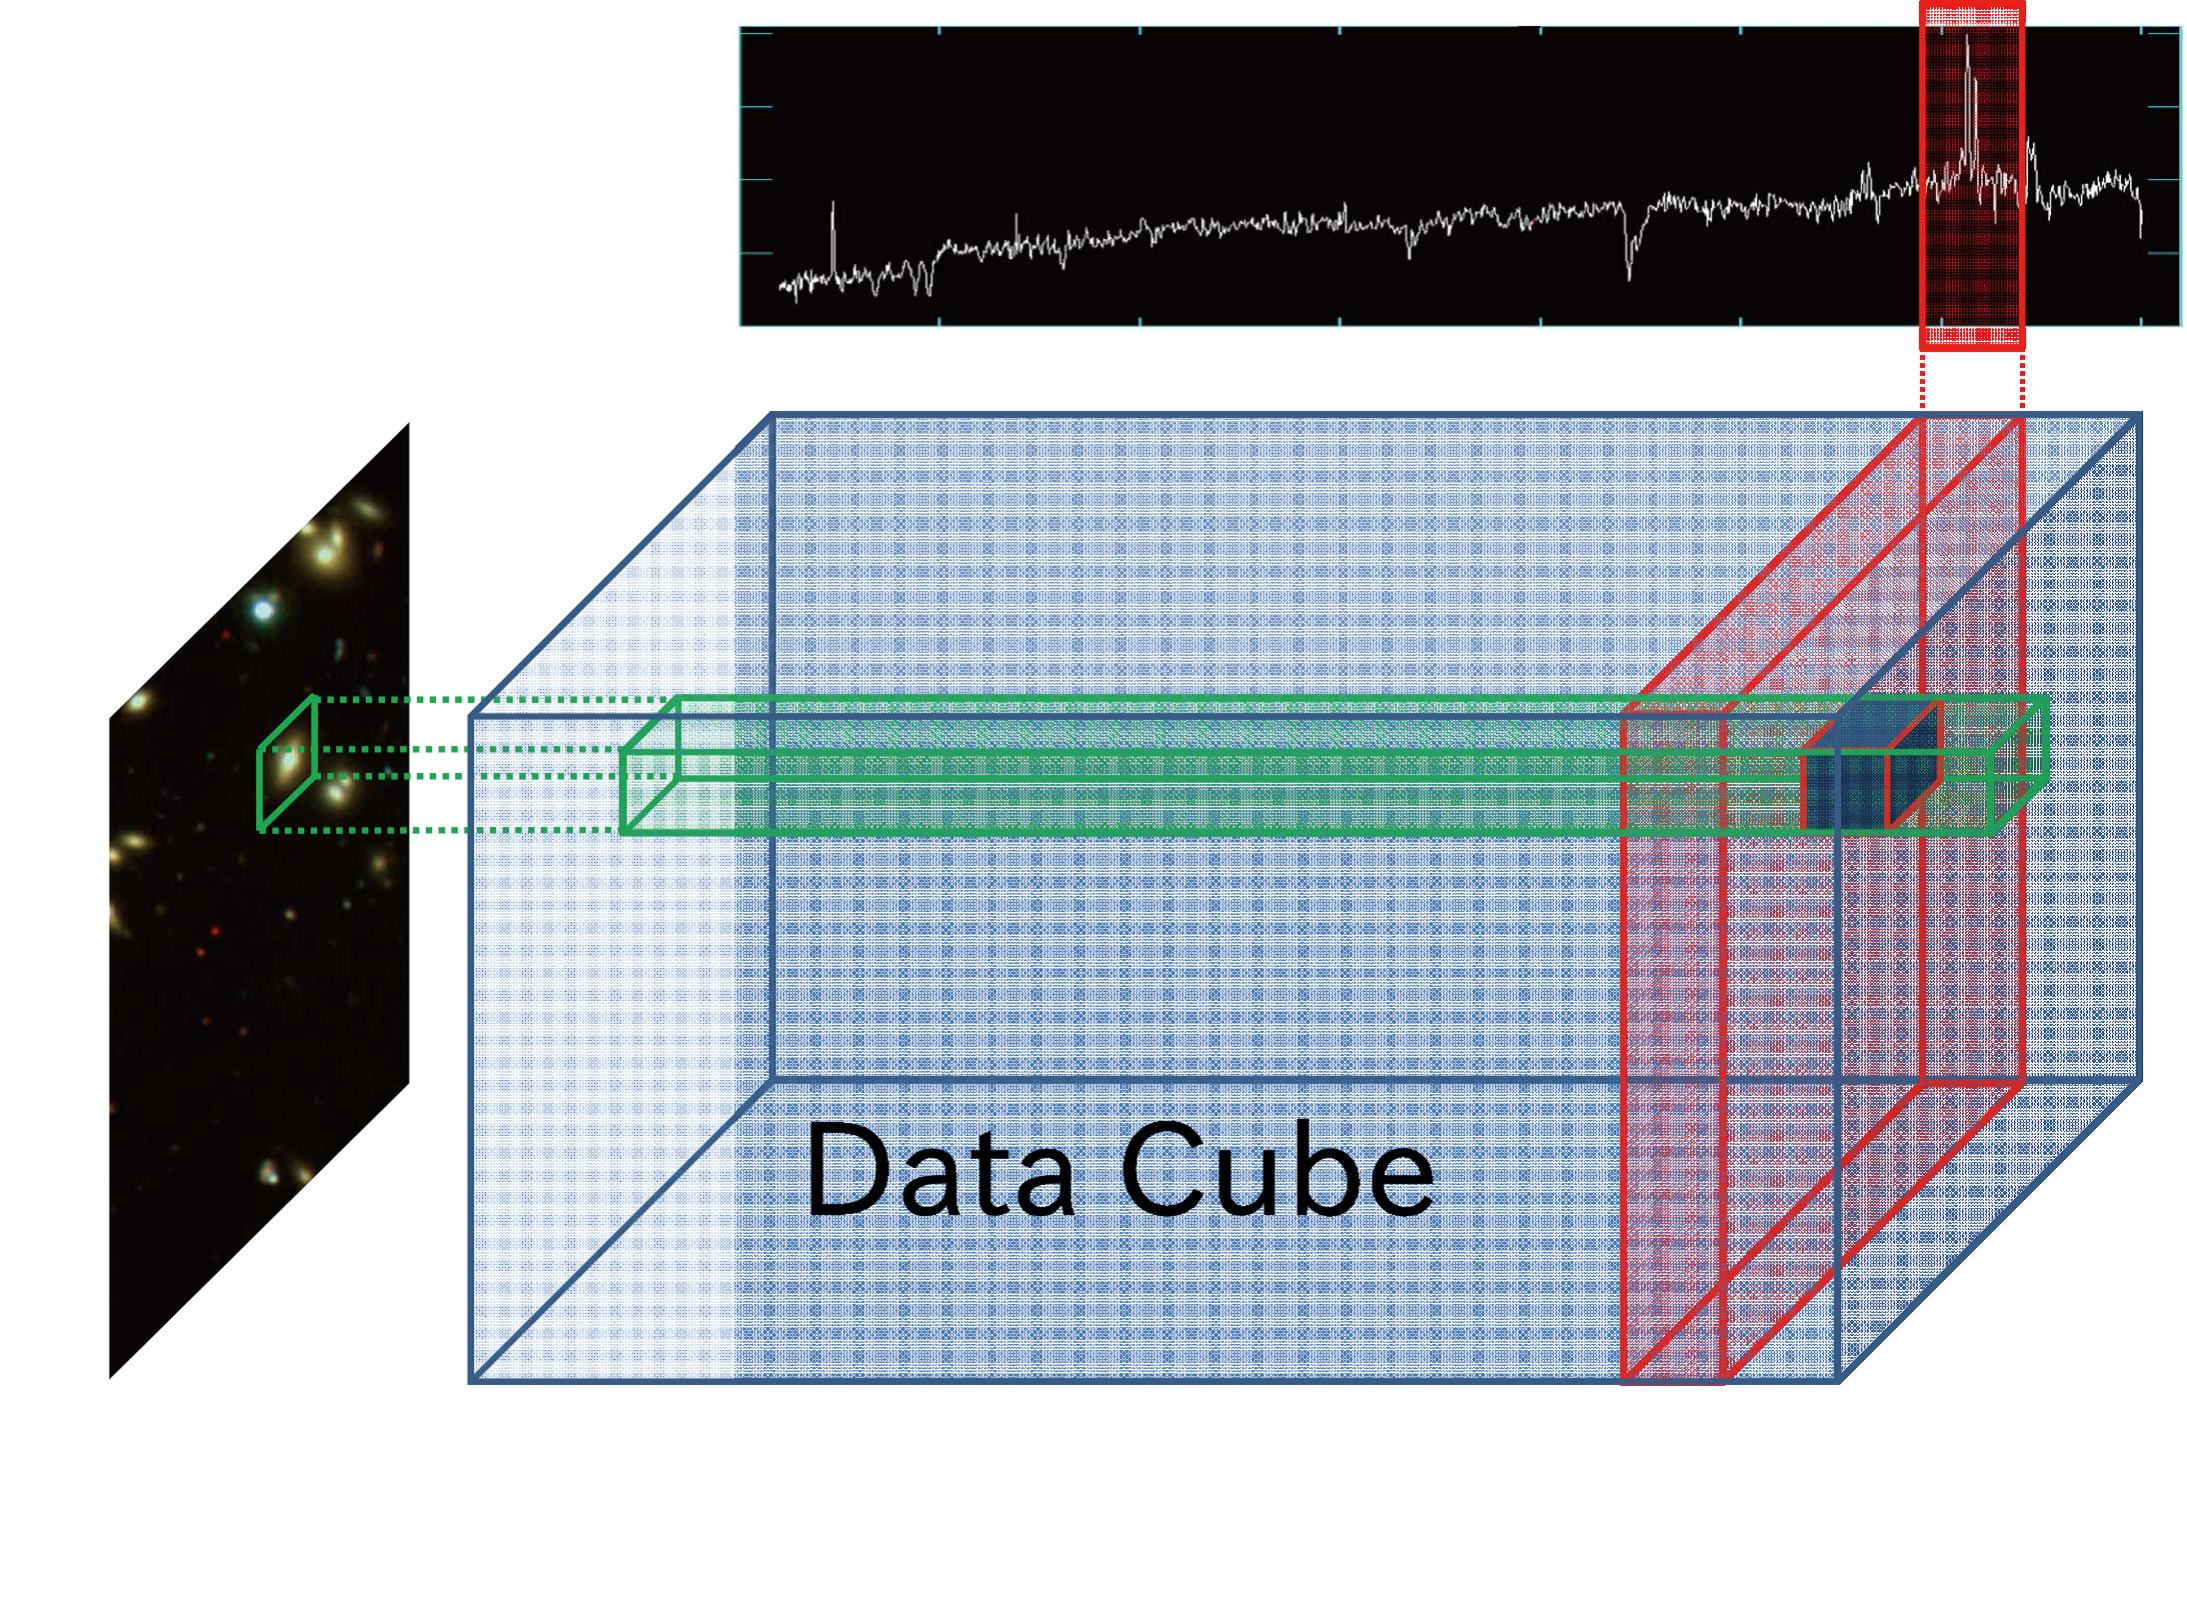
\includegraphics[width=0.45\textwidth]{images/cube.png}
    \caption{Estructura de cubos de datos de ALMA \cite{dent20132}}
    \label{fig:cube}
\end{figure}

En cuanto a los formatos de datos en astronomía, todos se rigen por una estructura
similar compuesta por metadatos (información que describe los datos) más datos
binarios. ALMA posee dos modelos de datos especiales:
\begin{description}
    \item[ALMA Science Data Model:] \hfill \\
        Formato en XML diseñado para guardar los metadatos obtenidos del
        proceso de observación y generar un link hacia los datos binarios.
    \item[Measurement Set:] \hfill \\
        Formato basado en tablas binarias (1 principal y varias secundarias),
        el que también guarda metadata y datos binarios. Este formato se usa
        para realizar reducción y procesamiento en el 
        Common Astronomy Software Applications (CASA), 
        software creado por NRAO\footnote{\url{http://casa.nrao.edu/}} para estos fines.
\end{description}

\subsection{El Observatorio Virtual Chileno}
%VO con datos de ALMA.
Chile, siendo uno de los países con más actividad astronómica en el mundo, no poseía hasta
hace un año un VO. Por el momento, ALMA tampoco tiene posee servicios
compatibles con los protocolos y estándares de otros VO, por lo que es un desafío
plantear necesidades y requerimientos de este tipo de sistema.
Si bien la comunidad internacional lleva varios años trabajando y puliendo
los observatorios virtuales y sus estándares, cada nuevo telescopio e
instrumento impone nuevos desafíos y oportunidades de desarrollo. 
Este es el caso de los datos de ALMA, que introduce el problema del
\emph{Big Data} como dilema presente, lo que requiere equipar al 
observatorio virtual que albergue sus datos de tecnología de punta 
e investigación de frontera en sus herramientas.

%Resumen de lo importante del paper.
Este paper tiene como objetivo introducir al lector a la arquitectura general de
Observatorios Virtuales y en particular al desarrollo actual que está
realizando el Chilean Virtual Observatory (ChiVO), desde el punto de vista de
desarrollo de software. Además se presentará el estado actual y cómo se
abordaron las restricciones y problemáticas que imponen los datos de ALMA.

%\subsection{IVOA Standards} No creo que sea necesario
